\chapter{Additional Tables}
\begin{table}[h]
    \centering
\begin{tabular}{lll|c}
Branching Factor $b$ & Distribution Factor $k$ & Growth Factor $g$ & Allocated Seeds $S_0$ \\ \hline
\multirow[c]{8}{*}{{\cellcolor[HTML]{F7FBFF}}} 5 & \multirow[c]{4}{*}{{\cellcolor[HTML]{F7FBFF}}} 5 & {\cellcolor[HTML]{F7FBFF}} 1.2 & 0 \\
{\cellcolor[HTML]{F7FBFF}}  & {\cellcolor[HTML]{F7FBFF}}  & {\cellcolor[HTML]{CCDFF1}} 1.3 & 1 \\
{\cellcolor[HTML]{F7FBFF}}  & {\cellcolor[HTML]{F7FBFF}}  & {\cellcolor[HTML]{82BBDB}} 1.4 & 2 \\
{\cellcolor[HTML]{F7FBFF}}  & {\cellcolor[HTML]{F7FBFF}}  & {\cellcolor[HTML]{58a9d6}} 1.5 & 3 \\
{\cellcolor[HTML]{F7FBFF}}  & \multirow[c]{4}{*}{{\cellcolor[HTML]{6AAED6}}} 6 & {\cellcolor[HTML]{F7FBFF}} 1.2 & 4 \\
{\cellcolor[HTML]{F7FBFF}}  & {\cellcolor[HTML]{6AAED6}}  & {\cellcolor[HTML]{CCDFF1}} 1.3 & 5 \\
{\cellcolor[HTML]{F7FBFF}}  & {\cellcolor[HTML]{6AAED6}}  & {\cellcolor[HTML]{82BBDB}} 1.4 & 6 \\
{\cellcolor[HTML]{F7FBFF}}  & {\cellcolor[HTML]{6AAED6}}  & {\cellcolor[HTML]{58a9d6}} 1.5 & 7 \\
\multirow[c]{8}{*}{{\cellcolor[HTML]{ABD0E6}}} 10 & \multirow[c]{4}{*}{{\cellcolor[HTML]{F7FBFF}}} 5 & {\cellcolor[HTML]{F7FBFF}} 1.2 & 8 \\
{\cellcolor[HTML]{ABD0E6}}  & {\cellcolor[HTML]{F7FBFF}}  & {\cellcolor[HTML]{CCDFF1}} 1.3 & 9 \\
{\cellcolor[HTML]{ABD0E6}}  & {\cellcolor[HTML]{F7FBFF}}  & {\cellcolor[HTML]{82BBDB}} 1.4 & 10 \\
{\cellcolor[HTML]{ABD0E6}}  & {\cellcolor[HTML]{F7FBFF}}  & {\cellcolor[HTML]{58a9d6}} 1.5 & 11 \\
{\cellcolor[HTML]{ABD0E6}}  & \multirow[c]{4}{*}{{\cellcolor[HTML]{6AAED6}}} 6 & {\cellcolor[HTML]{F7FBFF}} 1.2 & 12 \\
{\cellcolor[HTML]{ABD0E6}}  & {\cellcolor[HTML]{6AAED6}}  & {\cellcolor[HTML]{CCDFF1}} 1.3 & 13 \\
{\cellcolor[HTML]{ABD0E6}}  & {\cellcolor[HTML]{6AAED6}}  & {\cellcolor[HTML]{82BBDB}} 1.4 & 14 \\
{\cellcolor[HTML]{ABD0E6}}  & {\cellcolor[HTML]{6AAED6}}  & {\cellcolor[HTML]{58a9d6}} 1.5 & 15 \\
\multirow[c]{8}{*}{{\cellcolor[HTML]{58a9d6}}} 15 & \multirow[c]{4}{*}{{\cellcolor[HTML]{F7FBFF}}} 5 & {\cellcolor[HTML]{F7FBFF}} 1.2 & 16 \\
{\cellcolor[HTML]{58a9d6}}  & {\cellcolor[HTML]{F7FBFF}}  & {\cellcolor[HTML]{CCDFF1}} 1.3 & 17 \\
{\cellcolor[HTML]{58a9d6}}  & {\cellcolor[HTML]{F7FBFF}}  & {\cellcolor[HTML]{82BBDB}} 1.4 & 18 \\
{\cellcolor[HTML]{58a9d6}}  & {\cellcolor[HTML]{F7FBFF}}  & {\cellcolor[HTML]{58a9d6}} 1.5 & 19 \\
{\cellcolor[HTML]{58a9d6}}  & \multirow[c]{4}{*}{{\cellcolor[HTML]{6AAED6}}} 6 & {\cellcolor[HTML]{F7FBFF}} 1.2 & 20 \\
{\cellcolor[HTML]{58a9d6}}  & {\cellcolor[HTML]{6AAED6}}  & {\cellcolor[HTML]{CCDFF1}} 1.3 & 21 \\
{\cellcolor[HTML]{58a9d6}}  & {\cellcolor[HTML]{6AAED6}}  & {\cellcolor[HTML]{82BBDB}} 1.4 & 22 \\
{\cellcolor[HTML]{58a9d6}}  & {\cellcolor[HTML]{6AAED6}}  & {\cellcolor[HTML]{58a9d6}} 1.5 & 23 \\
\end{tabular}
    \caption{This table shows how the initial seed parameter $S_0$ of artificial game trees is allocated for Experiment~2, which is described in Subsection \ref{subsec:Exp2:Trees}. Based on the parameter values of a tree, we assign the value $s$ from 0 to 23, as read from the table above. Then the ranges of values $S_0$ for the trees included in the experiment are computed as $S_0 = 762391543368789717+24i + s$, where $i$ are all integer values from 0 to 499 inclusive. As such, a unique seed is assigned to each tree, for the total of 12\thsep000 trees included in Experiment~2.}
    \label{tab:SeedAllocationExp2}
\end{table}

\begin{table}[htbp]
\centering
\begin{tabular}{cc}
%
\begin{tabular}{l|llll}
Variant & Cost & Size & Time & Trees \\
\hline
\rowcolor{gray!50}
B* & 1 & 1 & 1 & 22\thsep179 \\
\rowcolor{white}
B*-alt & 1.05 & 1.08 & 1.05 & 22\thsep071 \\
B*$^2$ & 2.70 & 0.16 & 2.29 & 22\thsep177 \\
B*$^2$-alt & 2.99 & 0.17 & 2.69 & 22\thsep176 \\
df-B* & 23.14 & 0.02 & 93.54 & 15\thsep256 \\
df-B*-alt & 22.97 & 0.03 & 94.48 & 15\thsep461
\end{tabular}
%
&
%
\begin{tabular}{l|llll}
Variant & Cost & Size & Time & Trees \\
\hline
B* & 0.95 & 0.93 & 0.95 & 22\thsep071 \\
\rowcolor{gray!50}
B*-alt & 1 & 1 & 1 & 22\thsep161 \\
\rowcolor{white}
B*$^2$ & 2.72 & 0.15 & 2.38 & 22\thsep157 \\
B*$^2$-alt & 2.64 & 0.16 & 2.28 & 22\thsep159 \\
df-B* & 22.06 & 0.02 & 91.40 & 15\thsep256 \\
df-B*-alt & 22.10 & 0.02 & 93.58 & 15\thsep460
\end{tabular}
%
\\
(a) Trees solved by \textbf{B*}
&
(b) Trees solved by \textbf{B*-alt}
\bigskip\\
%
\begin{tabular}{l|llll}
Variant & Cost & Size & Time & Trees \\
\hline
B* & 0.37 & 6.15 & 0.44 & 22\thsep177 \\
B*-alt & 0.37 & 6.53 & 0.42 & 22\thsep157 \\
\rowcolor{gray!50}
B*$^2$ & 1 & 1 & 1 & 23\thsep048 \\
\rowcolor{white}
B*$^2$-alt & 1.05 & 1.04 & 1.10 & 22\thsep965 \\
df-B* & 14.77 & 0.19 & 74.30 & 15\thsep257 \\
df-B*-alt & 14.70 & 0.19 & 75.35 & 15\thsep462
\end{tabular}
%
&
%
\begin{tabular}{l|llll}
Variant & Cost & Size & Time & Trees \\
\hline
B* & 0.33 & 5.82 & 0.37 & 22\thsep176 \\
B*-alt & 0.38 & 6.36 & 0.44 & 22\thsep159 \\
B*$^2$ & 0.96 & 0.97 & 0.91 & 22\thsep965 \\
\rowcolor{gray!50}
B*$^2$-alt & 1 & 1 & 1 & 23\thsep049 \\
\rowcolor{white}
df-B* & 14.52 & 0.18 & 73.51 & 15\thsep257 \\
df-B*-alt & 14.51 & 0.19 & 74.95 & 15\thsep462
\end{tabular}
%
\\
(c) Trees solved by \textbf{B*}$^2$
&
(d) Trees solved by \textbf{B*}$^2$\textbf{-alt}
\bigskip\\
%
\begin{tabular}{l|llll}
Variant & Cost & Size & Time & Trees \\
\hline
B* & 0.04 & 41.35 & 0.01 & 15\thsep256 \\
B*-alt & 0.05 & 44.21 & 0.01 & 15\thsep256 \\
B*$^2$ & 0.07 & 5.33 & 0.01 & 15\thsep257 \\
B*$^2$-alt & 0.07 & 5.42 & 0.01 & 15\thsep257 \\
\rowcolor{gray!50}
df-B* & 1 & 1 & 1 & 15\thsep257 \\
\rowcolor{white}
df-B*-alt & 0.53 & 0.87 & 0.67 & 15\thsep132
\end{tabular}
%
&
%
\begin{tabular}{l|llll}
Variant & Cost & Size & Time & Trees \\
\hline
B* & 0.04 & 39.31 & 0.01 & 15\thsep461 \\
B*-alt & 0.05 & 41.35 & 0.01 & 15\thsep460 \\
B*$^2$ & 0.07 & 5.16 & 0.01 & 15\thsep462 \\
B*$^2$-alt & 0.07 & 5.22 & 0.01 & 15\thsep462 \\
df-B* & 1.89 & 1.15 & 1.49 & 15\thsep132 \\
\rowcolor{gray!50}
df-B*-alt & 1 & 1 & 1 & 15\thsep462
\end{tabular}
%
\\
(e) Trees solved by \textbf{df-B*}
&
(f) Trees solved by \textbf{df-B*-alt}
\end{tabular}
\caption{These tables show the relative performance of 6 B* variants, based on the results of Experiment 1, as described in Subsection \ref{subsec:ResultsExp1}. The ``Cost'', ``Size'', and ``Time'' columns show the ratios of the number of expansions, the number of nodes, and the duration of runs, relative to the variant in the highlighted row. Ratios of means are computed only over the set of trees which were solved by all iterations of both variants. The ``Trees'' column shows the number of trees in each set.}
\label{tab:RelativePerformance}
\end{table}

\chapter{Additional Details}
\section{Seed Allocation Experiment 1}
\label{sec:SeedAllocationExp1}
Subsection \ref{subsec:Exp1:Trees} describes how trees are initialised for Experiment~1. However, the values for the Initial Seed $S_0$ are determined for each tree individually. The seed allocation for trees in Experiment~1 uses a similar table to Table \ref{tab:SeedAllocationExp2}. However, this table would be too large to include, as there are 648 unique parameter combinations for the trees of Experiment~1.
Seeds are similarly assigned to Experiment~2, with the addition of the Relevance Chance parameter~$r$ (see Chapter \ref{cht:ArtificialGameTrees}).
The Relevance Chance column is included on the right side of all other parameter columns in the table, in the same order as the columns of Table \ref{tab:nodeLimitsExp2}. Seeds are then computed as $S_0 = 6623708332940258033 + 648i + s$, where $i$ are all integer values from 0 to 39 inclusive, and $s$ is incrementally assigned from 0 to 647 to each of the 648 unique parameter combinations.
The procedure thus assigns a unique seed to each of the 25\thsep920 trees included in Experiment~1.

\FloatBarrier
\chapter{Additional Figures}
\begin{figure}[htbp]
	\centering
	\ifMonochrome
	
\includegraphics[scale=0.7]
	{figures/graphs/monochrome/fig1TimePerExpandedSolvedByAnyBstar.pdf}
	\else
	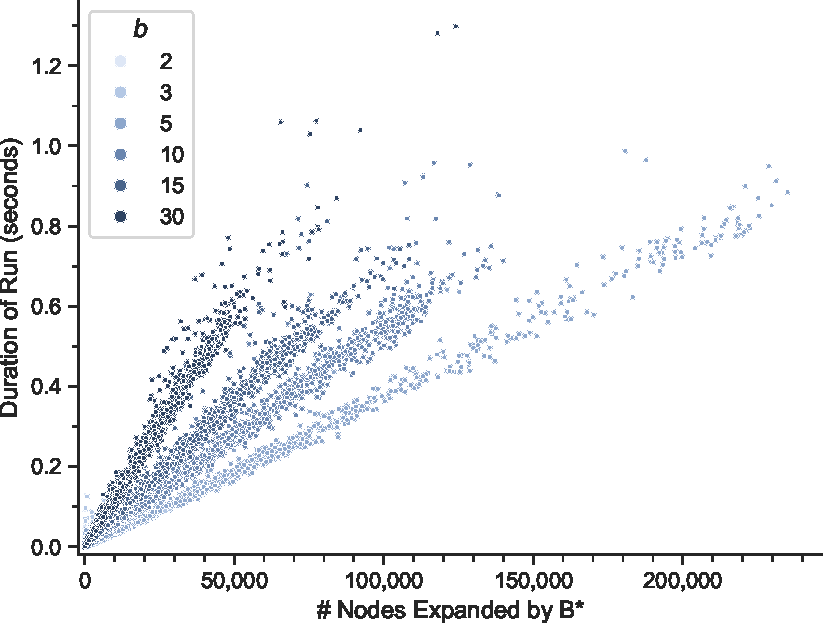
\includegraphics[scale=0.7]
	{figures/graphs/colour/fig1TimePerExpandedSolvedByAnyBstar.pdf}
	\fi
	\caption{This figure shows the duration of a run against the number of expansions for all runs solved by \textbf{B*} or \textbf{B*-alt}, from Experiment 1 (see Subsection \ref{subsec:ResultsExp1}). Runs displayed are categorised by the branching factor of the tree, which is negatively correlated with the number of expansions per second ($r\approx-0.54$).}
	\label{fig:Exp1TimePerExpandedSolvedByAnyBstar}
\end{figure}
%
\begin{figure}[htbp]
	\centering
	\ifMonochrome
	
\includegraphics[scale=0.7]
	{figures/graphs/monochrome/fig1TimePerExpandedSolvedByAnyBstarSQ.pdf}
	\else
	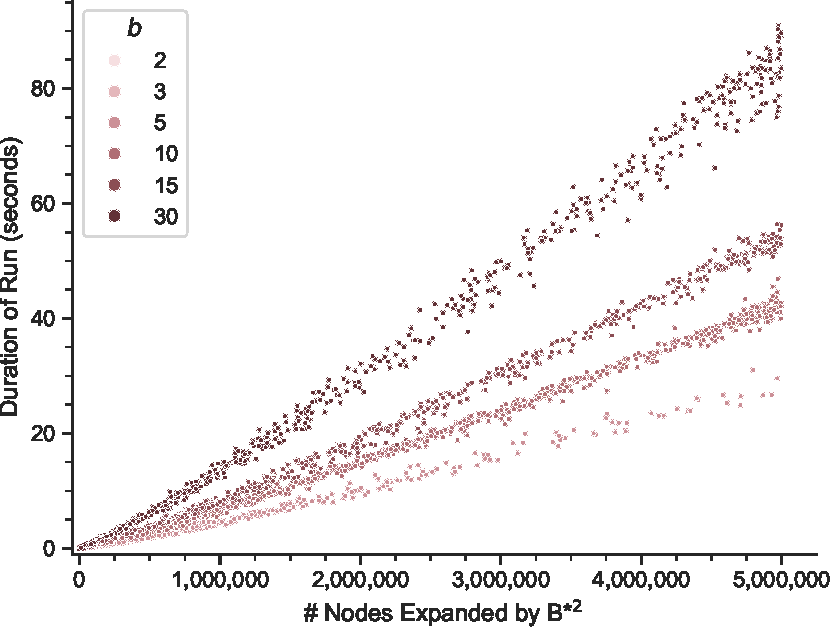
\includegraphics[scale=0.7]
	{figures/graphs/colour/fig1TimePerExpandedSolvedByAnyBstarSQ.pdf}
	\fi
	\caption{This figure shows the duration of a run against the number of expansions for all runs solved by \textbf{B*}$^2$ or \textbf{B*}$^2$\textbf{-alt}, for Experiment 1 (see Subsection \ref{subsec:ResultsExp1}). Runs displayed are categorised by the branching factor of the tree, which is negatively correlated with the number of expansions per second ($r\approx -0.62$).}
	\label{fig:Exp1TimePerExpandedSolvedByAnyBstarSQ}
\end{figure}
%
\begin{figure}[htbp]
	\centering
	\ifMonochrome
	
\includegraphics[scale=0.7]
	{figures/graphs/monochrome/fig1TimePerExpandedSolvedByAnyDfBstar.pdf}
	\else
	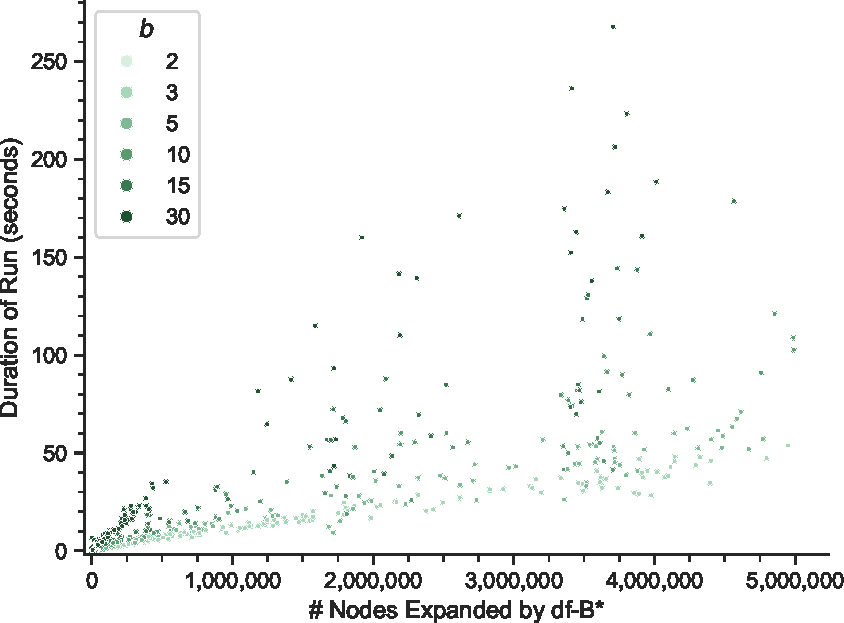
\includegraphics[scale=0.7]
	{figures/graphs/colour/fig1TimePerExpandedSolvedByAnyDfBstar.pdf}
	\fi
	\caption{This figure shows the duration of a run against the number of expansions for all runs solved by \textbf{df-B*} or \textbf{df-B*-alt}, for Experiment 1 (see Subsection \ref{subsec:ResultsExp1}). Runs displayed are categorised by the branching factor of the tree, which is not correlated with the number of expansions per second ($r\approx -0.03$).}
	\label{fig:Exp1TimePerExpandedSolvedByAnyDfBstar}
\end{figure}